\chapter{Testes e Resultados}
\label{ch::testes}

%\section{Introdução}
%\label{sec::testes:intro}
Deve ser assumido que durante toda a sequência de testes feita e registada, a aplicação foi compilada em \textbf{modo \textit{debug}} (no qual o programa retorna informação de \textit{debugging} útil no processo).

\section{Secções?}
A analisar\ldots


\begin{table}[!htbp]
	\centering
	\caption[Tempos de renderização em \acs{CPU}]{Tempo para a renderização de uma única \textit{frame} com recurso à \acs{CPU} para diferentes números de \textit{threads}. Os testes foram realizados no computador \textit{desktop} listado na Tabela \ref{tab::hardware}.}
	\label{tab::render_cpu}
	\begin{tabular}{r r r}
		\toprule
		\multirow{2}{*}{\textbf{Threads}} & \multicolumn{2}{c}{\textbf{Tempo}} \\
		\cline{2-3}
		 & Segundos & h:m's'' \\
		\midrule
		1 &  7087 & 01:58'07'' \\
		2 &  5984 & 01:39'44'' \\
		4 &  7566 & 02:06'06'' \\
		6 & 10414 & 02:53'34'' \\
		\bottomrule
	\end{tabular}
\end{table}


\begin{figure}[!htbp]
	\centering
	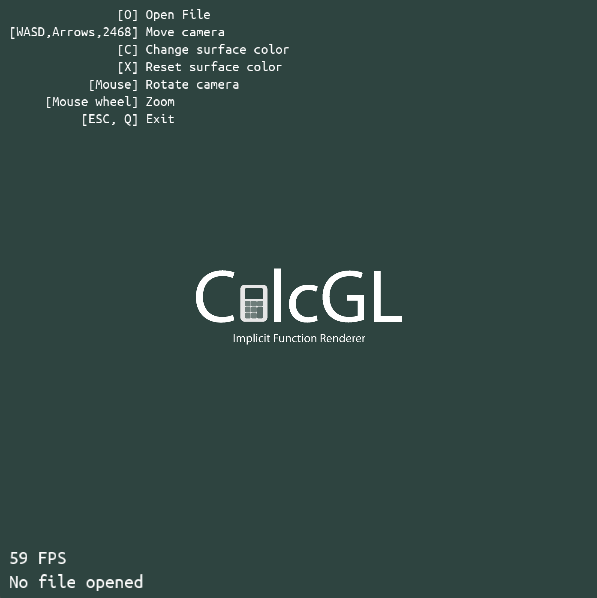
\includegraphics[width=.8\textwidth]{home}
	\caption[Ecrã inicial da aplicação]{Ecrã inicial da aplicação \theapp.}
	\label{fig::home}
\end{figure}

\begin{figure}[!htbp]
	\centering
	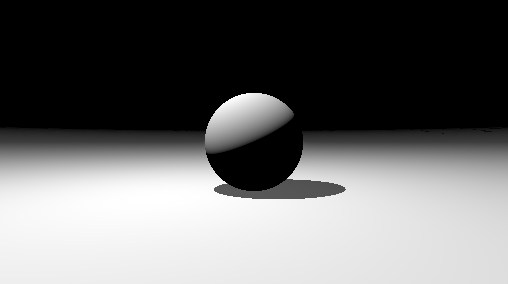
\includegraphics[width=.8\textwidth]{spheresphere}
	\caption[Teste do algoritmo de \textit{sphere tracing}]{Teste do algoritmo de \textit{sphere tracing} no \textit{website} \url{shadertoy.com} de uma esfera e um plano.}.
	\label{fig::spheresphere}
\end{figure}

\begin{figure}[!htbp]
	\centering
	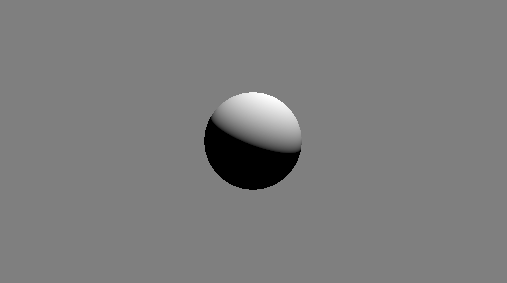
\includegraphics[width=.8\textwidth]{ashalgosphere}
	\caption[Teste do algoritmo naïve]{Teste do algoritmo naïve no \textit{website} \url{shadertoy.com} de uma esfera.}
	\label{fig::ashalgosphere}
\end{figure}

\begin{figure}[!htbp]
	\centering
	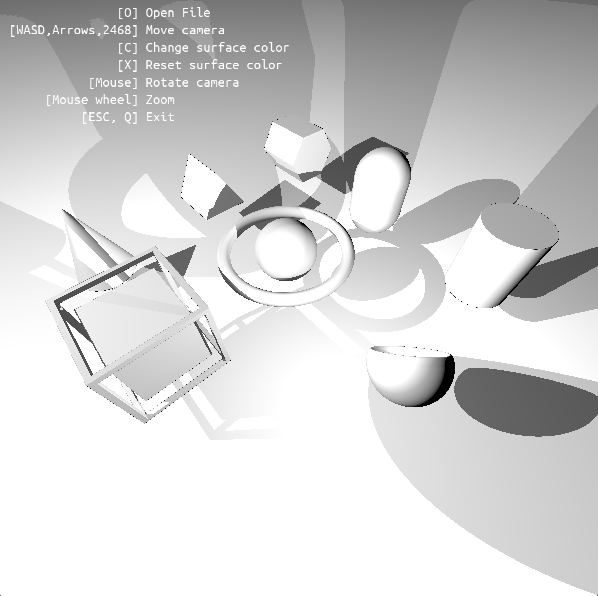
\includegraphics[width=.8\textwidth]{sphereoriginal}
	\caption[Nove objetos com \textit{sphere tracing} no \theapp]{Renderização de nove objetos no \theapp~usando o algoritmo de \textit{sphere tracing}.}
	\label{fig::sphereoriginal}
\end{figure}

\begin{figure}[!htbp]
	\centering
	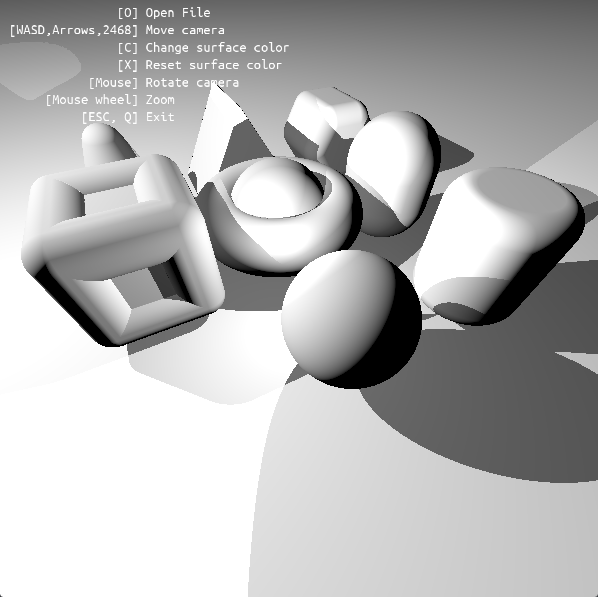
\includegraphics[width=.8\textwidth]{spheresmooth}
	\caption[Nove objetos com \textit{sphere tracing} e suavização no \theapp]{Renderização de nove objetos no \theapp~usando o algoritmo de \textit{sphere tracing} com um fator de suavização $s$ dependente do tempo de execução $t$, em particular $s = \cos(t)$.}
	\label{fig::spheresmooth}
\end{figure}

\begin{figure}[!htbp]
	\centering
	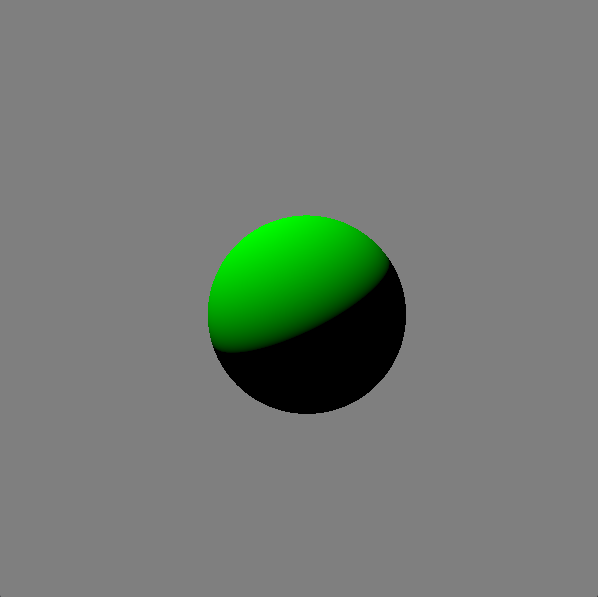
\includegraphics[width=.8\textwidth]{calcglsphere}
	\caption[Esfera no \theapp~com algoritmo naïve]{Esfera renderizada no \theapp, em fase inicial de testes, com o algoritmo naïve.}
	\label{fig::calcglsphere}
\end{figure}

\begin{figure}[!htbp]
	\centering
	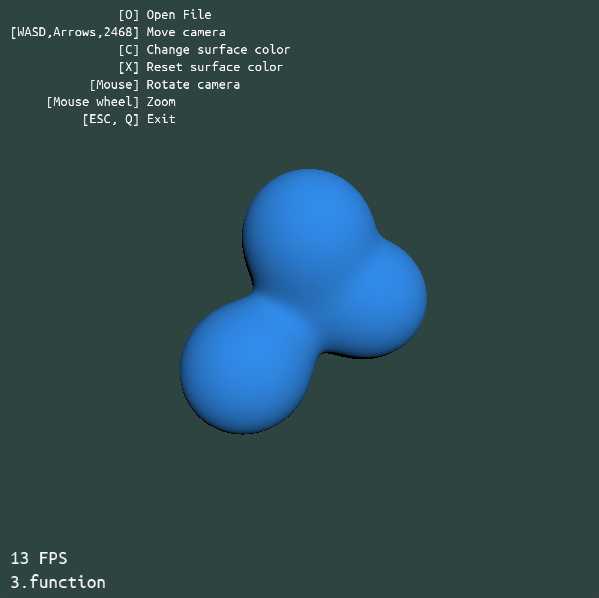
\includegraphics[width=.8\textwidth]{calcglpisurf}
	\caption[Superfície $\Pi$ no \theapp~com algoritmo naïve]{Superfície $\Pi$ renderizada no \theapp~com algoritmo naïve.}
	\label{fig::calcglpisurf}
\end{figure}

\begin{figure}[!htbp]
	\centering
	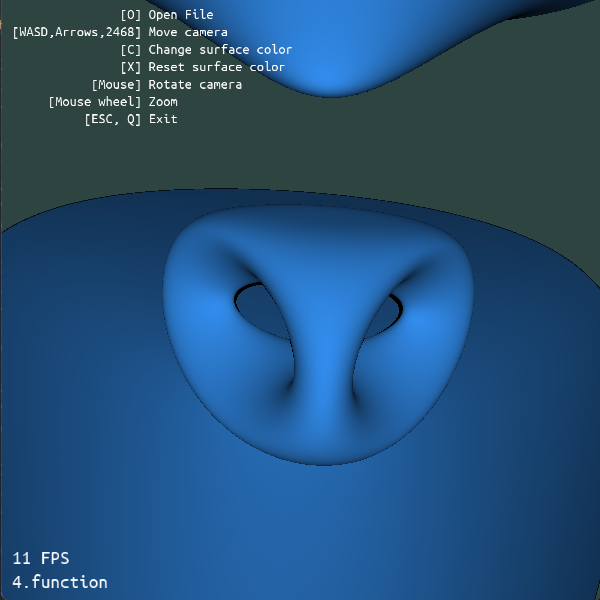
\includegraphics[width=.8\textwidth]{calcglgenus}
	\caption[\textit{Genus} no \theapp~com algoritmo naïve]{\textit{Genus} renderizado no \theapp~com algoritmo naïve.}
	\label{fig::calcglgenus}
\end{figure}


%\section{Conclusões}
%\label{sec::testes:conc}
